\documentclass[../main.tex]{subfiles}
\graphicspath{{figures/}{../figures/}}

\begin{document}
\todo[color=green!30]{完成问题一模型的建立(sections/q1\_build)}
\noindent \textbf{Step 1 坐标系的建立}

\begin{itemize}
\item \textbf{定日镜场坐标系的建立}
\end{itemize}

\par 为定义整个定日镜场中所有物体的位置以及位置之间的相关关系,我们建立以圆形场形定日镜场的中心$O$为原点,  
正东方向为$x$轴正方向,正北方向为$y$轴正方向,垂直地面向上为$z$轴正方向的定日镜场坐标系。在此坐标系下,记定日镜中心坐标为 \( P_i(x_i, y_i, z_i) \) 。 
  \begin{figure}[H]
    \centering
    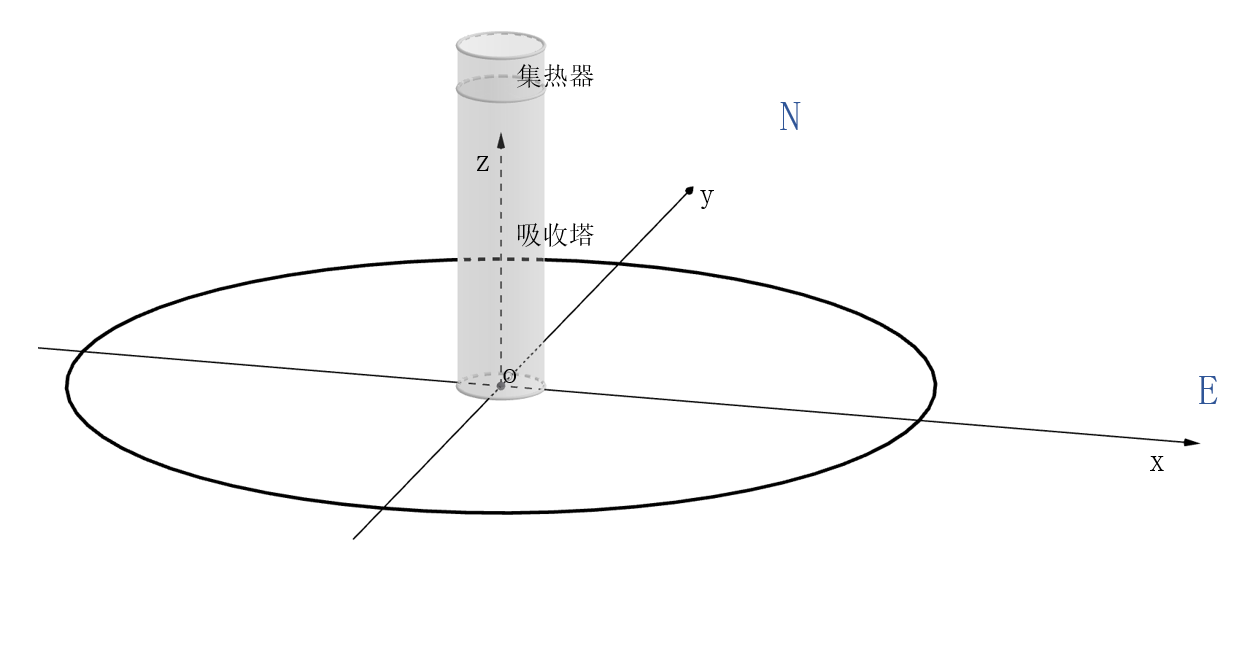
\includegraphics[width=.6\textwidth]{1}
    \caption{定日镜场大地坐标系}
    \label{1.1}
\end{figure}
    \begin{itemize}
  \item \textbf{定日镜面坐标系的建立}
  \end{itemize}
\par 为便于描述定日镜面上的各点及其位置关系,我们建立以定日镜中心$O_i$为坐标原点,过原点垂直镜面向外的法向量为$z$轴正方向,过原点平行于定日镜水平转轴面向镜面水平向左为$x$轴正方向,过原点垂直于定日镜水平转轴面向镜面向下为$y$轴正方向的定日镜面坐标系。
\begin{figure}[H]
\centering
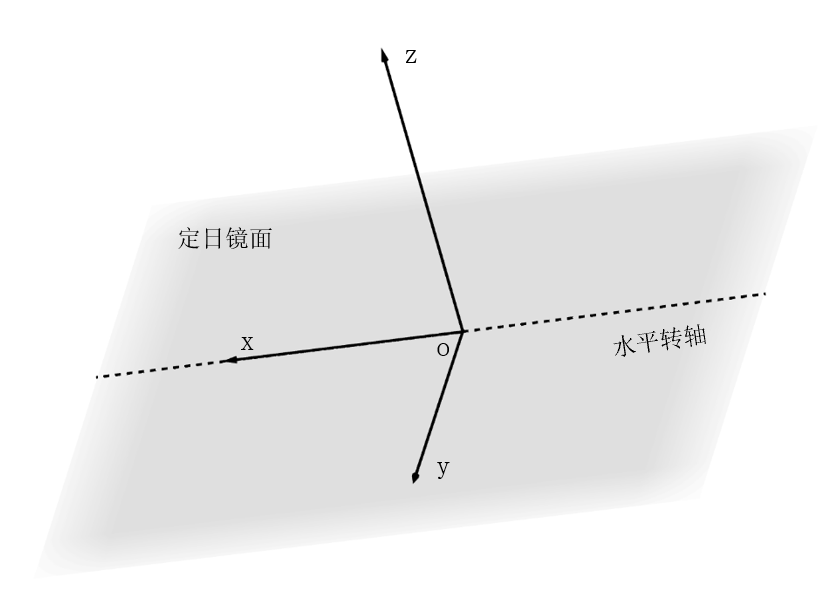
\includegraphics[width=.6\textwidth]{2}
\caption{定日镜面坐标系}
\label{1.2}
\end{figure}
\begin{itemize}
\item \textbf{光锥坐标系的建立}
\end{itemize}
\par 太阳光并非平行光线,而是具有一定锥形角的一束锥形光线,其中锥形光束的中心入射光线与水平面的夹角为太阳高度角。因此我们需要通过建立光锥坐标系从而分析锥型光束中的入射光线。
\par 光锥坐标系以锥形入射光线在定日镜上的落点为原点$O_s$,$z$轴正方向与锥形光束的中心入射光线相反;$y$轴所在直线满足其在地面投影与定日镜场中心指向正北方向的射线平行,且以其靠近北极点的一端为$y$轴正方向;以\( \overrightarrow{O_sx}=\overrightarrow{O_sz}\times \overrightarrow{O_sy}\)为$x$轴正方向. 

在光锥坐标系下,通过径向角$\theta _l$(即锥形光束内的入射光线与$z$轴的夹角,范围为 \([0, 4.65\ \mathrm{mrad}]\))和方向角$\beta _l$(即光线在光锥坐标系 \( xoy \) 面的投影与 \( y\) 轴之间的夹角 ,范围为 \([0, 2\pi]\))可以表示锥形光束内每条入射光线的方向向量:  
\begin{align}    \label{1.3}
\vec{e}_l=\left( -\sin \theta _l\sin \beta _l,\,\,-\sin \theta _l\cos \beta _l,\,\,-\cos \theta _l \right) .
\end{align} 

\noindent \textbf{Step 2 定日镜法向量}
\par \textbf{(1) 入射光线方向向量}
\par 在定日镜场坐标系下,我们通过太阳高度角和方位角确定太阳的位置,进而得到定日境场坐标系下的入射光线方向向量。
\begin{figure}[H]
\centering
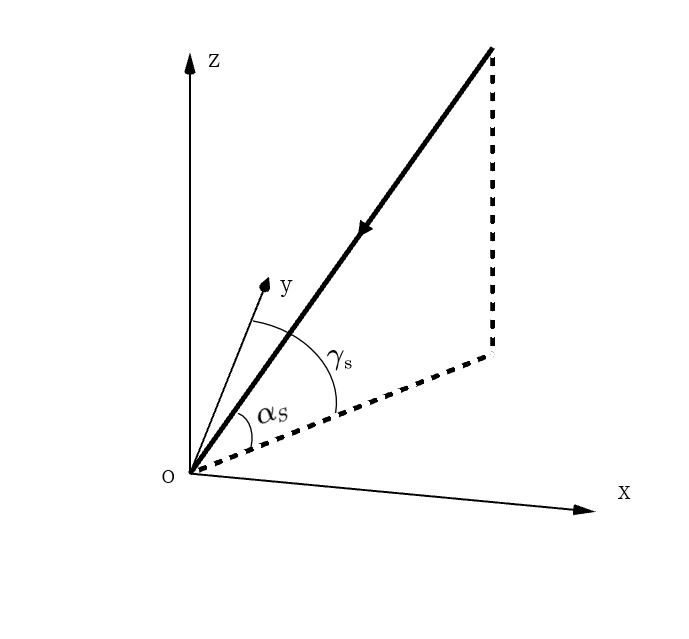
\includegraphics[width=.6\textwidth]{3}
\caption{入射光线在定日镜场坐标系下的位置关系示意图}
\label{1.2}
\end{figure} 
\begin{itemize}
\item \textbf{太阳高度角 $\alpha_{\text{s}}$}
\end{itemize}
\par 太阳高度角指太阳到定日镜场坐标系原点的连线与地平面的夹角,其计算公式为:
\begin{align}    \label{1.4}
\sin \alpha _{\text{s}}=\cos \delta \cos \varphi \cos \omega +\sin \delta \sin \varphi \quad \left( \alpha _{\text{s}}\in \left[ 0,\frac{\pi}{2} \right] \right) 
\end{align}
\par 其中,$\delta$ 为太阳赤纬角即太阳光线与地球赤道平面的夹角 ,$\gamma$ 为当地纬度,规定北纬为正,$\omega$ 为太阳时角,描述太阳在一天中相对于当地正午位置的角度偏移,根据附录可知太阳赤纬角和太阳时角计算公式为:
\begin{align}    \label{1.5}
\sin\delta = \sin\frac{2\pi D}{365} \sin\left(\frac{2\pi}{360}(23.45)\right)
\end{align}
\begin{align}    \label{1.6}
\omega = \frac{\pi}{12}(ST - 12)
\end{align}
\par 其中, $D$ 为以春分作为第 0 天起算的天数,$ST$ 为当地时间(h)。
\begin{itemize}
\item \textbf{太阳方位角 $ \gamma _{\text{s}}$}
\end{itemize}
\par 太阳方位角即从$y$轴正方向起始,顺时针旋转至太阳入射光线在地平面上的投影所转过的角度,其相关计算公式为:
\begin{align}    \label{1.7}
\cos \gamma _{\text{s}}=\frac{\sin \delta -\sin \alpha _{\text{s}}\sin \varphi}{\cos \alpha _{\text{s}}\cos \varphi}\quad \left( \gamma _{\text{s}}\in \left[ 0,2\pi \right] \right) 
\end{align}
\par 根据太阳高度角$\alpha_{\text{s}}$及太阳赤纬角$\delta$和当地纬度$\varphi$即可求得。

\begin{itemize}
\item \textbf{入射光线方向向量}
\end{itemize}
\par 如图所示,已知太阳方位角和太阳高度角即可确定入射光线单位向量$\vec{e}_j =(x_j, y_j, z_j)$,其表达式如下:
\begin{align}\label{1.8}
\begin{cases}
x_j=-\cos \alpha _s\sin \gamma _s\\
y_j=-\cos \alpha _s\cos \gamma _{\mathrm{s}}\\
z_j=-\sin \alpha _s\\
\end{cases},
\end{align}
\par 即:
\begin{align}\label{1.9}
\vec{e}_{j}=(-\cos \alpha _s\sin \gamma _{\mathrm{s}}, -\cos \alpha _s\cos \gamma _{\mathrm{s}}, -\sin \alpha _s).
\end{align}
\par \textbf{(2) 反射光线方向向量}
\par 定日镜在工作时,控制系统根据太阳的位置实时控制定日镜的法向量,使得入射光线经定日镜中心反射后指向集热器中心。由于集热器中心的高度为吸收塔高度,吸收塔高度为 80m,集热器高度为 8m,则集热器中心离地面的高度$H_T=84$,从而集热器中心的坐标为$(0,0,H_T)$。题目已经给定定日镜中心位置$P_{i}(x_i,y_i,z_i)$,因此反射光线方向向量$\vec{e}_{\text{k}}=(x_k,y_k,z_k)$为:
\begin{align}    \label{1.10}
\vec{e}_{\text{k}} = \frac{(-x_i, -y_i, H_T - z_i)}{\sqrt{x_i^2 + y_i^2 + (H_T - z_i)^2}}.
\end{align}
\par \textbf{(3) 定日镜单位法向量}
\par 已知定日镜入射光线单位向量、反射光线单位向量,则我们可以得到定日镜法向量$\vec{e}=(e_x,e_y,e_z)$:
\begin{align}    \label{1.11}
\vec{e} = \frac{\vec{e}_{\text{k}} - \vec{e}_{\text{j}}}{|\vec{e}_{\text{k}} - \vec{e}_{\text{j}}|}
\end{align}



  \noindent \textbf{Step 3 坐标系之间的转换}
\par 为了更加准确描述镜场坐标系、镜面坐标系、锥形坐标系下各点及向量之间的相互关系,我们需要将三个坐标系进行转换,进行坐标系之间的转换。
\par \textbf{(1) 定日镜俯仰角$\alpha_{P_{i}}$和方位角$\gamma_{P_{i}}$}

\par 进行坐标系转换前,我们需要知道定日镜俯仰角 $\alpha_{P_{i}}$和方位角 $\gamma_{P_{i}}$,定日镜在工作时,控制系统会根据太阳的位置调整定日镜的法向,因此我们可以根据定日镜的法向量确定定日镜的俯仰角 $\alpha_{P_{i}}$ 和方位角 $\gamma_{P_{i}}$ ,关系如图所示
   \begin{figure}[H]
    \centering
    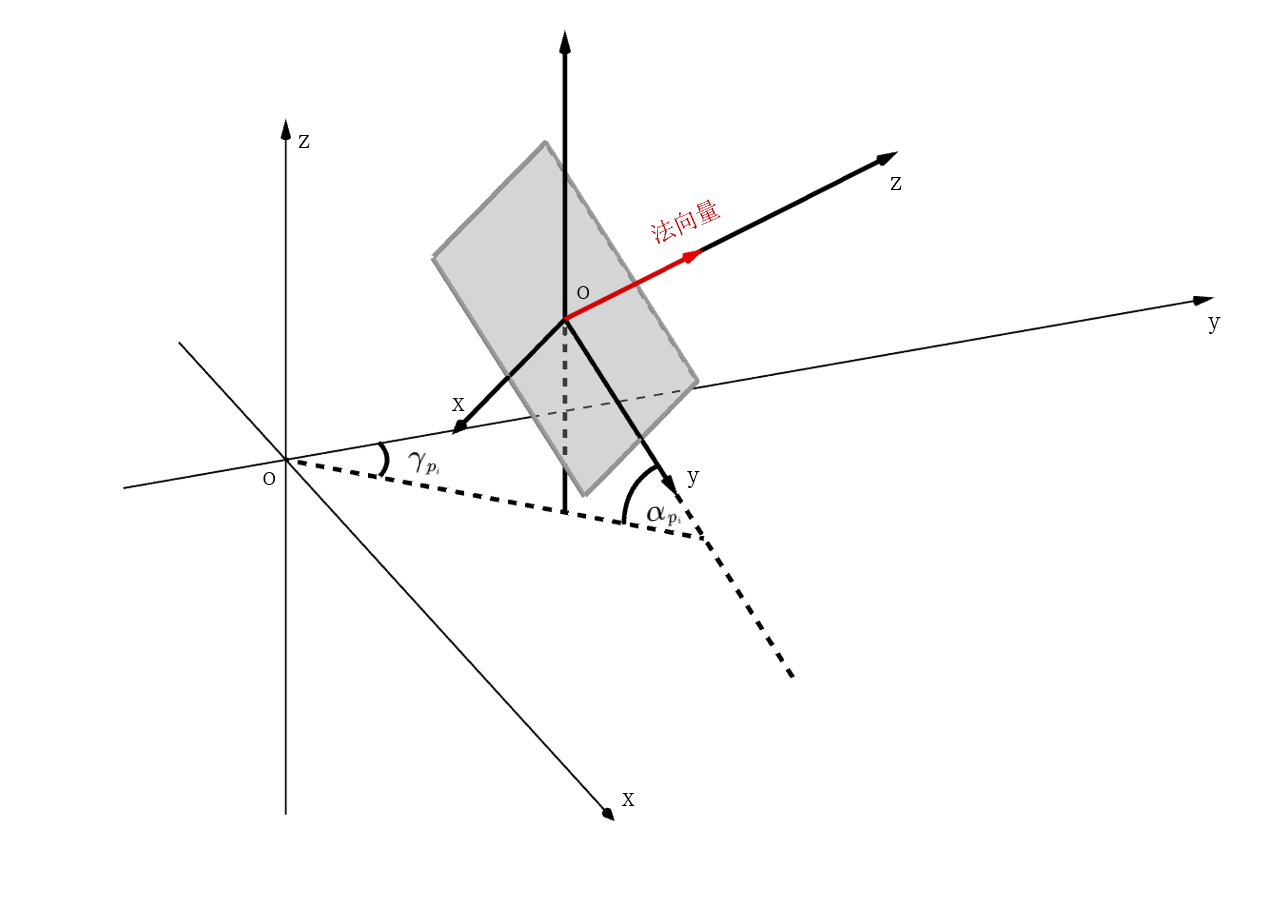
\includegraphics[width=.8\textwidth]{4}
    \caption{定日镜法向量与俯仰角和方位角关系示意图}
    \label{1.12}
\end{figure} 


\begin{itemize}
\item \textbf{定日镜俯仰角 $\alpha_{P_{i}}$ }
\end{itemize}
\par 定日镜的俯仰角即定日镜与地平面之间的夹角。如\cref{1.12}所示,其为定日镜法向量与定日镜场系$z$轴之间的夹角,因此定日镜俯仰角相关公式:
\begin{align}    \label{1.13}
\cos\alpha_{P_i} = e_z,\quad \alpha_{P_{i}} \in [0, \frac{\pi}{2}]
\end{align}

\begin{itemize}
  \item \textbf{定日镜方位角 $\gamma_{P_{i}}$  }
  \end{itemize}
  \par 定日镜的方位角即以定日镜中心在地面上的投影为原点,从正北方向顺时针旋转至定日镜法向量在水平面的投影所形成的夹角,因此定日镜方位角相关公式:
    \begin{align}    \label{1.14}
\tan\gamma_{P_i} = \frac{e_{x}}{e_{y}}
\end{align}               


\par \textbf{(2) 坐标系之间的相互转换}
\begin{itemize}
\item \textbf{定日镜面坐标系与定日镜场坐标系的转换}
\end{itemize}
\par 如\cref{1.12}所示,先面向$x$轴(定日镜面坐标系)负方向,将定日镜面坐标系绕$x$轴(定日镜面坐标系)逆时针方向旋转$\alpha _{P_i}$,再面向$z$轴(定日镜面坐标系)负方向,绕\(z\)轴(定日镜面坐标系)逆时针旋转$\gamma_{P_i}$,得到新的坐标系的坐标轴与定日镜场坐标系的坐标轴平行.此时的旋转矩阵为:
\begin{align}\label{1.15}
T_i=\left[ \begin{matrix}
\cos \gamma _{P_i}&		-\sin \gamma _{P_i}&		0\\
\sin \gamma _{P_i}&		\cos \gamma _{P_i}&		0\\
0&		0&		1\\
\end{matrix} \right] \left[ \begin{matrix}
1&		0&		0\\
0&		\cos \alpha _{P_i}&		-\sin \alpha _{P_i}\\
0&		\sin \alpha _{P_i}&		\cos \alpha _{P_i}\\
\end{matrix} \right] 
\end{align}
设定日镜面坐标系的坐标原点$O_i$在定日镜场坐标系下的坐标为$(x_{O_i},y_{O_i},z_{O_i})^T$,$P$点在定日镜面坐标系下的坐标为$(x,y,z)^T$,在定日镜场坐标系下的坐标为$(x',y',z')^T$,则
\begin{align}\label{eq:100.1}
\left[ \begin{matrix}
x'\\
y'\\
z'\\
\end{matrix} \right] =T_i\left[ \begin{matrix}
x\\
y\\
z\\
\end{matrix} \right]+\left[ \begin{matrix}
x_{O_i}\\
y_{O_i}\\
z_{O_i}\\
\end{matrix} \right].
\end{align}

\begin{itemize}
\item \textbf{光锥坐标系与定日镜场坐标系的转换}
\end{itemize}
\par 光锥坐标系入射光束的中心入射光线方向相反, 且中心入射光线与地平面的夹角为太阳高度角 $\alpha _s$。注意到光锥坐标系的 $y$ 轴在镜面坐标系上的投影与镜面坐标系的 $y$ 轴平行, 且中心入射光线在地面的投影与正北方向之间的夹角为太阳方位角 $\gamma_S$。
\begin{figure}[H]
\centering
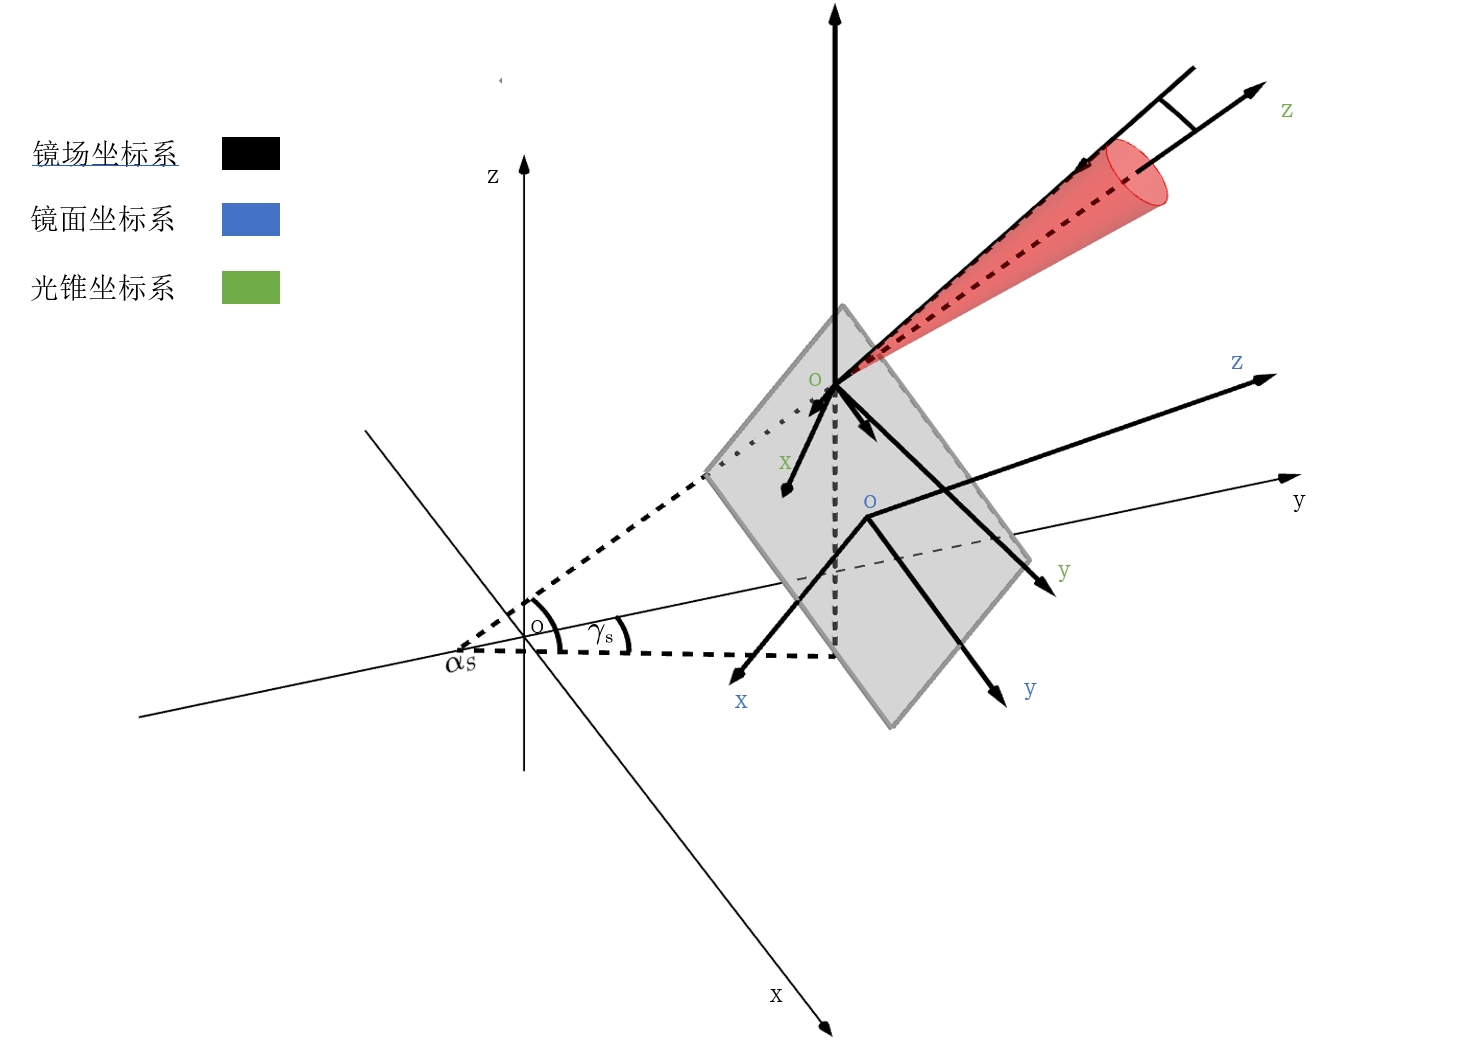
\includegraphics[width=.9\textwidth]{5}
\caption{光锥坐标系与定日镜场坐标系关系示意图}
\label{1.16}
\end{figure}
\par 因此, 先面向$x$轴负方向,将光锥坐标系先绕$x$轴逆时针旋转$\frac{\pi}{2}-\alpha_s$, 再面向$z$轴负方向,绕 $z$ 轴逆时针旋转 $\gamma_s$,得到新的坐标系的坐标轴与定日镜场坐标系的坐标轴平行.此时的旋转矩阵为:
\begin{align}    \label{1.17}
T_s=\left[ \begin{matrix}
\cos \gamma _s&		-\sin \gamma _s&		0\\
\sin \gamma _s&		\cos \gamma _s&		0\\
0&		0&		1\\
\end{matrix} \right] \left[ \begin{matrix}
1&		0&		0\\
0&		\sin \alpha _s&		-\cos \alpha _s\\
0&		\cos \alpha _s&		\sin \alpha _s\\
\end{matrix} \right] .
\end{align}
设光锥坐标系的坐标原点$O_i$在定日镜场坐标系下的坐标为$(x_{O_s},y_{O_s},z_{O_s})^T$,$P$点在光锥坐标系下的坐标为$(x,y,z)^T$,在定日镜场坐标系下的坐标为$(x',y',z')^T$,则
\begin{align}\label{eq:100.2}
\left[ \begin{matrix}
x'\\
y'\\
z'\\
\end{matrix} \right] =T_s\left[ \begin{matrix}
x\\
y\\
z\\
\end{matrix} \right]+\left[ \begin{matrix}
x_{O_s}\\
y_{O_s}\\
z_{O_s}\\
\end{matrix} \right]  .
\end{align}

\noindent \textbf{Step 4 定日镜场年平均光学效率\(\bar{\eta}\)}
\par 记定日镜场中总共有$M$块定日镜,第 \(i\) 块定日镜在第 \(j\) 个月21日第 \(t_k\) 个时刻的光学效率为 \(\eta_{ijk}\),其中$j\in \{1,2,\cdots,12\},t_1=9,t_2=10.5,t_3=12,t_4=13.5,t_5=15$.则年平均光效率 \(\bar{\eta}\) 为:
\begin{align}\label{1.50}
\bar{\eta}=\frac{\sum\limits_{i=1}^M{\sum\limits_{j=1}^{12}{\sum\limits_{k=1}^5{\eta _{ijk}}}}}{60M}
\end{align}
\par 因此,我们需要得知每块定日镜的光学效率,根据附录提供的定日镜光学效率公式:
\begin{align}\label{1.18}
\eta =\eta _{\text{sb}}\eta _{\cos}\eta _{\text{at}}\eta _{trunc}\eta _{\text{ref}}
  \end{align}
\par 可以得知定日镜光学效率与阴影遮挡效率$\eta_{\text{sb}}$、余弦效率$\eta_{\text{cos}}$、大气透射率$\eta_{\text{at}}$、集热器截断效率$\eta_{\text{trunc}}$、镜面反射率$\eta_{\text{ref}}$有关。
\par \textbf{(1) 阴影遮挡效率 $\eta_{\text{sb}}$}
\par 根据附录可知,阴影遮挡效率与阴影遮挡损失有关。阴影遮挡损失由两部分组成,分别是吸收塔与集热器组成的圆柱体对太阳光线的遮挡和前排定日镜对后排定日镜光线的遮挡。
\begin{itemize}
  \item \textbf{吸收塔与集热器组成的圆柱体对太阳光线的遮挡}
\end{itemize}
\par 如图所示,当太阳照射至定日镜的入射光线被吸收塔与集热器遮挡时,太阳光线照射不到定日镜上,会造成一定的阴影遮挡损失 。
 \begin{figure}[H]
\centering
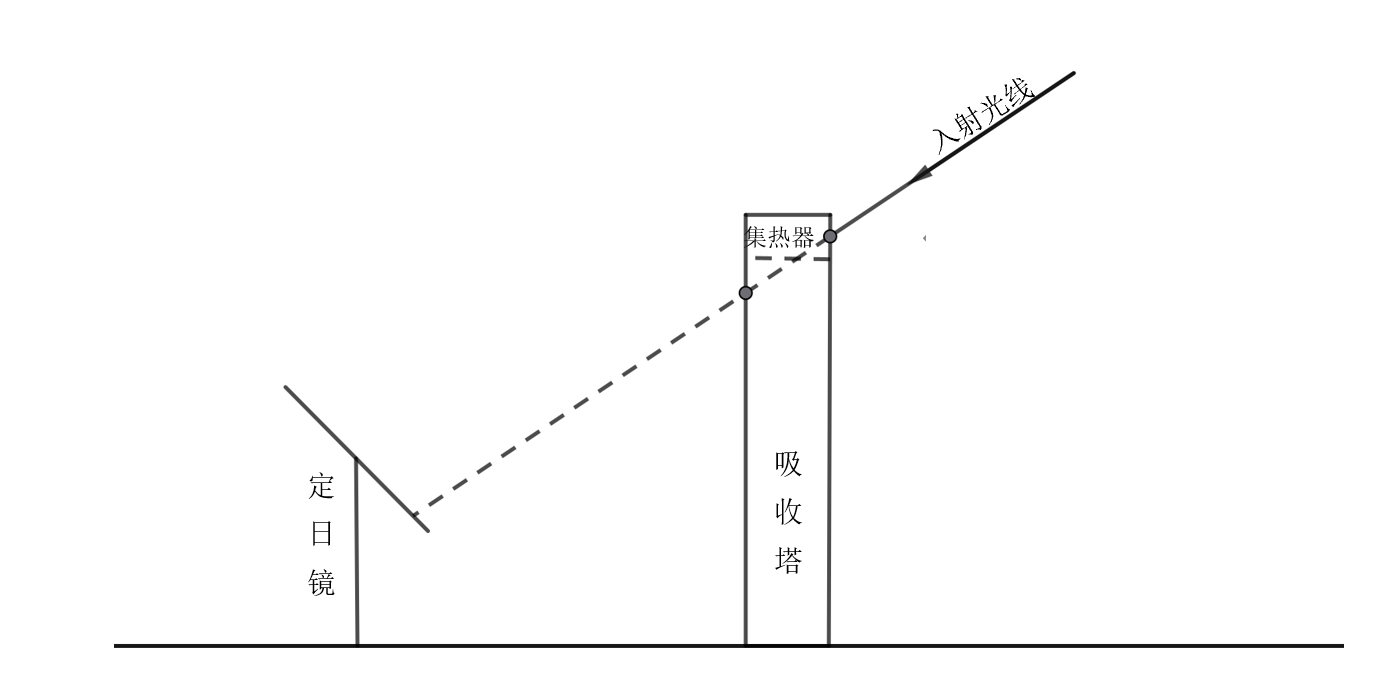
\includegraphics[width=.9\textwidth]{6}
\caption{吸收塔与集热器对太阳光线的遮挡示意图}
\label{1.19}
\end{figure}
\par 由\eqref{1.3}式知太阳入射光束中任一入射光线方向向量在光锥坐标系下的坐标为
\begin{align}\label{1.20}
\vec{e}_l=\left( -\sin \theta _l\sin \beta _l,\,\,-\sin \theta _l\cos \beta _l,\,\,-\cos \theta _l \right)=(x_l, y_l, z_l)
\end{align}
利用\eqref{eq:100.2}可得其在定日镜场坐标系下的坐标为
\begin{align}    \label{1.21}
\left[ \begin{matrix}
x_l'\\
y_l'\\
z_l'\\
\end{matrix} \right] =T_s\left[ \begin{matrix}
-\sin \theta_l \sin \beta_l\\
-\sin \theta_l \cos \beta_l\\
-\cos\theta_l\\
\end{matrix} \right]
\end{align}
\par 在镜面坐标系下,记入射光线在镜面上的着落点为 \( M_0(x_0, y_0, z_0) \),将其转换为镜场坐标系下的坐标 \( M_0'(x_0', y_0', z_0') \),即:
\begin{align}    \label{1.22}
\left[ \begin{array}{c}
x_{0}^{\prime}\\
y_{0}^{\prime}\\
z_{0}^{\prime}\\
\end{array} \right] =T_i\left[ \begin{array}{c}
x_0\\
y_0\\
z_0\\
\end{array} \right] +\left[ \begin{array}{c}
x_{O_s}\\
y_{O_s}\\
z_{O_s}\\
\end{array} \right] 
\end{align}
\par 从而可得在镜场坐标系下的入射光线的直线方程为:
\begin{align}    \label{1.23}
\begin{cases}
x = x_0' + x_l' t \\
y = y_0' + y_l' t \\
z = z_0' + z_l' t \\
\end{cases}
\end{align}
\par 吸收塔和集热器表面的方程为:
\begin{align}\label{1.24}
\begin{cases}
x^2+y^2=R^2\\
0\leqslant z\leqslant h\\
\end{cases}.
\end{align}
\par 根据题目给定条件可知\( R = 3.5 \, \text{m} \)。 联立公式\eqref{1.23}\eqref{1.24},得到
\begin{align}    \label{1.25}
(x_{l}'^{2}+y_{l}'^{2})t^{2}+2(x_{0}'x_{l}'+y_{0}'y_{l}')t+(x_{0}'^{2}+y_{0}'^{2}-R^{2}) = 0
\end{align}
\par 其判别式为:
\begin{align}    \label{1.26}
\Delta=4(x_0'x_l' + y_0'y_l')^2 - 4(x_l'^2 + y_l'^2)(x_0'^2 + y_0'^2 - R^2)
\end{align}
\par 当\(\Delta \leqslant 0\)时,入射光线未被吸收塔与集热器组成的圆柱体遮挡;当\(\Delta >0\)时,入射光线与吸收塔横截面有两个不同交点,由\eqref{1.25}式可得这两个交点对应的参数$t_1,t_2$分别为
\begin{align}
t_1=\frac{-2(x_0'x_l'+y_0'y_l')+\sqrt{\Delta}}{2\left[ \left( x_{l}^{\prime} \right) ^2+\left( y_{l}^{\prime} \right) ^2 \right]},\quad t_2=\frac{-2(x_0'x_l'+y_0'y_l')-\sqrt{\Delta}}{2\left[ \left( x_{l}^{\prime} \right) ^2+\left( y_{l}^{\prime} \right) ^2 \right]}.
\end{align}
通过题目给定条件可知,吸收塔与集热器组成的圆柱体高度$h=88m$.因此当所有交点高度的最小值大于$h$,入射光线未被吸收塔与集热器组成的圆柱体遮挡;小于或等于$h$,入射光线被吸收塔与集热器组成的圆柱体遮挡。即:
\begin{align}\label{1.27}
\begin{cases} 
\Delta \leqslant 0 \hspace{0.5em} \text{未被遮挡} \\[6pt]
\Delta > 0 
\begin{cases} 
\min\{z_0' + z_1 t_1,\, z_0' + z_1 t_2\} > h & \quad \text{未被遮挡} \\[4pt]
\min\{z_0' + z_1 t_1,\, z_0' + z_1 t_2\} \leqslant h & \quad \text{被遮挡} 
\end{cases}
\end{cases}
\end{align}
\par 由\eqref{1.9}式知太阳入射光束中心入射光线方向向量(定日镜场坐标系下)为
\begin{align}\label{1.19}
\vec{e}_{j} = (-\cos\delta\sin\gamma_{s},\ -\cos\delta\cos\gamma_{s},\ -\sin\delta)=(x_j, y_j, z_j)
\end{align}
利用\eqref{eq:100.2}可得其在定日镜场坐标系下的坐标为
\begin{align}\label{1..21}
\left[ \begin{matrix}
x_j'\\
y_j'\\
z_j'\\
\end{matrix} \right] =T_s\left[ \begin{matrix}
-\cos\delta\sin\gamma_{s}\\
-\cos\delta\cos\gamma_{s}\\
-\sin\delta\\
\end{matrix} \right]
\end{align}
从而可得在镜场坐标系下的入射光线的直线方程为:
\begin{align}\label{1..23}
\begin{cases}
x = x_0' + x_j' t \\
y = y_0' + y_j' t \\
z = z_0' + z_j' t \\
\end{cases}
\end{align}
同理联立公式\eqref{1..23}\eqref{1.24},得到
\begin{align}\label{1..25}
(x_{j}'^{2}+y_{j}'^{2})t^{2}+2(x_{0}'x_{j}'+y_{0}'y_{j}')t+(x_{0}'^{2}+y_{0}'^{2}-R^{2}) = 0.
\end{align}
其判别式为:
\begin{align}\label{1..26}
\Delta'=4(x_0'x_j' + y_0'y_j')^2 - 4(x_j'^2 + y_j'^2)(x_0'^2 + y_0'^2 - R^2).
\end{align}
当$\Delta'>0$时,同理可得两个交点对应的参数$t_1',t_2'$分别为
\begin{align}
t_{1}^{\prime}=\frac{-2(x_0' x_j' +y_0' y_j' )+\sqrt{\Delta'}}{2\left[ \left( x_{j}^{\prime} \right) ^2+\left( y_{j}^{\prime} \right) ^2 \right]},\quad t_{2}^{\prime}=\frac{-2(x_0' x_j' +y_0' y_{j}^{\prime})-\sqrt{\Delta'}}{2\left[ \left( x_{j}^{\prime} \right) ^2+\left( y_{j}^{\prime} \right) ^2 \right]}.
\end{align}
同理可得太阳入射光束中心入射光线是否被吸收塔与集热器组成的圆柱体遮挡的判断条件:
\begin{align}\label{1..27}
\begin{cases} 
\Delta' \leqslant 0 \hspace{0.5em} \text{未被遮挡} \\[6pt]
\Delta' > 0 
\begin{cases} 
\min\{z_0' + z_j' t_1',\, z_0' + z_j' t_2'\} > h & \quad \text{未被遮挡} \\[4pt]
\min\{z_0' + z_j' t_1',\, z_0' + z_j' t_2'\} \leqslant h & \quad \text{被遮挡} 
\end{cases}
\end{cases}
\end{align}

\par 为了确定有多少入射光线被吸收塔与集热器组成的圆柱体遮挡,我们记第$w$个入射光线是否被遮挡为$a_1^w$,其为0,1向量,则
\begin{align}\label{1.28}
a_{1}^{2}=\begin{cases}
0,\text{第}w\text{个入射光线未被遮挡}\\
1,\text{第}w\text{个入射光线被遮挡}\\
\end{cases}.
\end{align}
\begin{itemize}
  \item \textbf{前排定日镜对后排定日镜光线的遮挡}
\end{itemize}
\par 当入射光线未被吸收塔与集热器组成的圆柱体遮挡时,我们需要考虑以下两种情况。
\par \textbf{1 前排定日镜对后排定日镜入射光线的遮挡}
\par 如图所示,当通过镜 \( A \) 上的某一点的入射光线所在的直线与镜面 \( B \) 有交点,则此入射光线被镜 \( A \) 遮挡,无法照射到镜 \( B \) 上,从而造成阴影遮挡损失。
\begin{figure}[H]
\centering
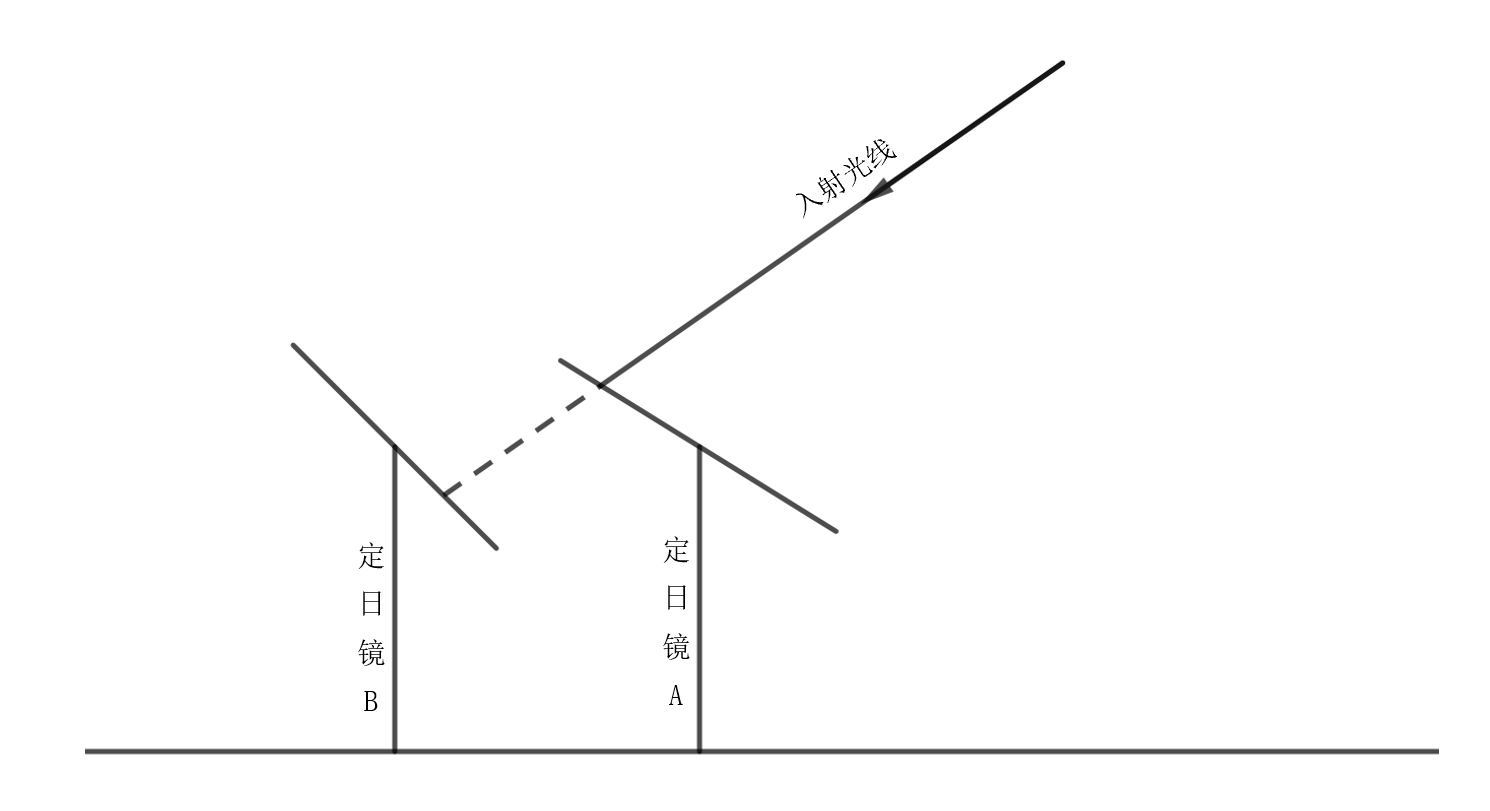
\includegraphics[width=.9\textwidth]{7}
\caption{入射光线遮挡示意图}
\label{1.29}
\end{figure}
\par 在镜面坐标系$A$下,取镜面 \( A \) 上一点 \( W_a\),设其坐标为$(x_a,y_a,z_a)$,将其转换为定日镜场坐标系下的坐标 \( (x_a', y_a', z_a') \),即
\begin{align}\label{1.30}
  W_a' = T_A W_a + P_A
\end{align}
\par 再将其转换为镜面坐标系 \( B \) 上的坐标:
\begin{align}\label{1.31}
 W_a'' = (T_B)^T (W_a' - P_B)=(x_a'', y_a'', z_a'')
\end{align}
\par 将太阳入射光束中任一入射光线在光锥坐标系下的方向向量$\vec{e}_l(x_l, y_l, z_l)$转换为定日镜镜场坐标系下的向量
\begin{align}    \label{1.32}
\vec{e}_l'=T_S\vec{e}_l=\left( x_l',y_l',z_l' \right) 
\end{align}
\par 再将其转换到定日镜面$B$坐标系中,即
\begin{align} \label{1.33}
  \vec{e}_l'' = (T_B)^T \vec{e}_l' = (x_l'', y_l'', z_l'')
\end{align}
 \par 记经过平面 $A$ 的入射光线上的点为 $(x, y, z)$,则在镜面 $B$ 坐标系下,入射光线可表示为:
\begin{align} \label{1.34}
 \begin{cases}
x = x_a'' + x_l'' t \\
y = y_a'' + y_l'' t \\
z = z_a'' + z_l'' t
\end{cases}
\end{align}
\par 设入射光线与 $B$ 镜(即镜面 $B$ 坐标系的 $xOy$ 平面)的交点为 $(m_l, n_l, 0)$,若 $-3 \leq m_l \leq 3$,$-3 \leq n_l \leq 3$,且此交点在定日镜场坐标系下的 $z$ 坐标$p_l$小于所取的镜面 $A$ 上的点在定日镜场坐标系下所对应的 $z$ 坐标 $z_a'$,则入射光线被镜 \( A \) 遮挡,无法照射到镜 \( B \) 上。
\par 将大地坐标系下的入射主光线方向向量$\vec{e}_j (x_j, y_j, z_j)$转换到定日镜面$B$坐标系中,即
\begin{align}    \label{1.32}
\vec{e}_j'=(T_B)^T\vec{e}_j=\left( x_j',y_j',z_j' \right) 
\end{align}
\par 同理,结合$ W_a''(x_a'', y_a'', z_a'')$求与$B$镜面的交点 $(m_l, n_l, 0)$进行判断。
\par 为了确定有多少入射光线被前排定日镜遮挡,我们记第$w$个入射光线是否被遮挡为$a_2^w$,其为0,1向量,则
\begin{align}    \label{1.33}
a_2^w = 
\begin{cases} 
0, & \text{else 未被遮挡} \\
1, & -3 \leq m_l \leq 3,\ -3 \leq n_l \leq 3,\ p_l < z_a'\ \text{被遮挡} 
\end{cases}
 \end{align}
\par \textbf{2 前排定日镜对后排定日镜反射光线的遮挡}
\par  如果前排定日镜未对后排定日镜入射光线遮挡,则考虑前排定日镜对后排定日镜反射光线的遮挡。如图所示,当通过镜 $A$ 上的某一点的入射光线所在直线与镜面 $B$ 相交,则反射光线被定日镜$A$ 遮挡,无法到达集热器上,从而造成阴影遮挡损失。
    \begin{figure}[H]
    \centering
    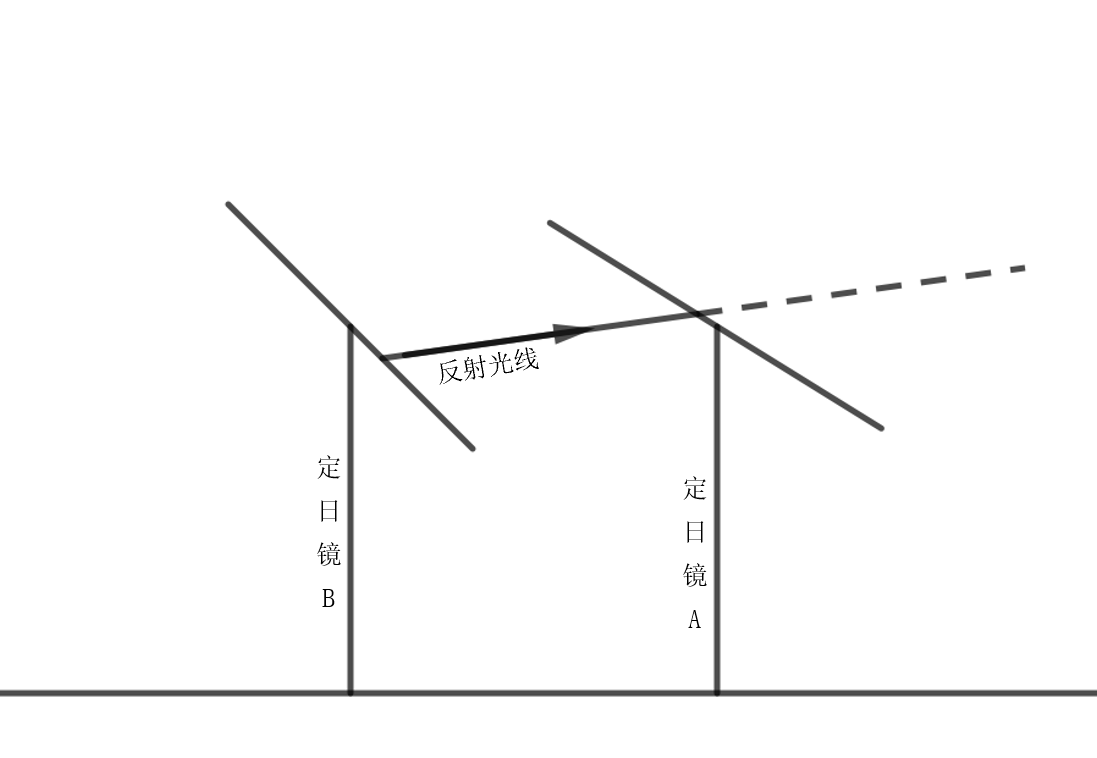
\includegraphics[width=.9\textwidth]{8}
    \caption{反射光线遮挡示意图}
    \label{1.29}
\end{figure}
\par 太阳光并非平行光线,而是具有一定锥形角的一束锥形光线,入射光束中经过定日镜反射后仍为一束锥形光线,且法向量为定日镜面的法向量$\vec{e}(e_x,e_y,e_z)$.因此,在定日镜场坐标系下,入射光束中的入射光线经过定日镜反射后的反射光线方向向量$\vec{e}_m(x_m, y_m, z_m)$为
\begin{align}  \label{1.30}
\vec{e}_m = \vec{e}_i' - 2 (\vec{e}_m \cdot \vec{e}) \vec{e}
\end{align}
\par 在镜面坐标系$A$下,取镜面 \( A \) 上一点 \( W_a (x_a,y_a,z_a) \),将其转换为定日镜场坐标系下的坐标 \( W_a' (x_a', y_a', z_a') \),即
\begin{align}\label{1.30}
   W_a' = T_A W_a + P_A
\end{align}
\par 再将其转换为镜面坐标系 \( B \) 上的坐标:
\begin{align}\label{1.31}
 W_a'' = (T_B)^T (W_a' - P_B)=(x_a'', y_a'', z_a'')
\end{align}
\par 将太阳入射光束经定日镜反射后的反射光束中任一反射光线在光锥坐标系下的方向向量$\vec{e}_r(x_r, y_r, z_r)$转换为定日镜场坐标系下的向量
\begin{align}    \label{1.32}
\vec{e}_r'=T_S\vec{e}_r=\left( x_r',y_r',z_r' \right) 
\end{align}
\par 再将其转换到定日镜面$B$坐标系中,即
\begin{align} \label{1.33}
  \vec{e}_r'' = (T_B)^T \vec{e}_r' = (x_r'', y_r'', z_r'')
\end{align}
 \par 记经过平面 $A$ 的反射光线上的点为 $(x, y, z)$,则在镜面 $B$ 坐标系下,反射光线可表示为:
\begin{align} \label{1.34}
 \begin{cases}
x = x_a'' + x_r'' t \\
y = y_a'' + y_r'' t \\
z = z_a'' + z_r'' t
\end{cases}
\end{align}
\par 设反射光线与 $B$ 镜(即镜面 $B$ 坐标系的 $xOy$ 平面)的交点为 $(m_r, n_r, 0)$,若 $-3 \leq m_r \leq 3$,$-3 \leq n_r \leq 3$,且此交点在定日镜场坐标系下的 $z$ 坐标$p_r$小于所取的镜面 $A$ 上的点在定日镜场坐标系下所对应的 $z$ 坐标 $z_a'$,则反射光线被镜 \( A \) 遮挡,无法照射到镜 \( B \) 上。
\par 将大地坐标系下的反射主光线方向向量$\vec{e}_k (x_k, y_k, z_k)$转换到定日镜面$B$坐标系中,即
\begin{align}    \label{1.32}
\vec{e}_k'=(T_B)^T\vec{e}_k=\left( x_k',y_k',z_k' \right) 
\end{align}
\par 同理,结合$ W_a''(x_a'', y_a'', z_a'')$求与$B$镜面的交点 $(m_r, n_r, 0)$进行判断。
\par 为了确定有多少反射光线被前排定日镜遮挡,我们记第$w$个反射光线是否被遮挡为$a_3^w$,其为0,1向量,则
\begin{align}    \label{1.33}
a_3^w = 
\begin{cases} 
0, & \text{else 未被遮挡} \\
1, & -3 \leq m_r \leq 3,\ -3 \leq n_r\leq 3,\ p_r < z_a'\ \text{被遮挡} 
\end{cases}
 \end{align}
\par 综上所述,记总光线数量为N,则阴影遮挡效率为
\begin{align}\label{1.34}
 \eta _{\text{sb}}=1-\frac{\sum_{w=1}^N{\left( a_{1}^{w}+a_{2}^{w}+a_{3}^{w} \right)}}{N}
\end{align}
\par \textbf{(2) 余弦效率 $\eta_{\text{cos}}$}
\par 余弦效率是指入射光线入射到定日镜平面时,定日镜接收到的实际光通量与假设光线垂直入射时接收到的光通量的比值。它主要反映了由于光线入射角的变化 ,导致接收面有效接收光能量的变化情况。设入射光线与法向量之间的夹角为$\theta $,则
\begin{align}\label{1.35}
  \eta_{\cos\theta} = \cos\theta = -\vec{e}_i \cdot \vec{e}
\end{align}
\par \textbf{(3) 大气透射率 $\eta_{\text{at}}$}
\par 大气透射率的产生是由于大气中的气体分子、气溶胶、水汽等成分对光线产生吸收和散射作用,导致部分光线能量被衰减,它反映了光线穿过大气层的传输效率。记镜面中心到集热器中心的距离为 $d_{\text{HR}}$(单位:$\text{m}$),则
\begin{align}\label{1.36}
 d_{\text{HR}} = \sqrt{(x_i)^2 + y_i^2 + (z_i - H_T)^2}
 \end{align}
\par 根据附录可知大气透射率计算公式为:
\begin{align}\label{1.36}
  \eta_{\text{at}} = 0.99321 - 0.0001176d_{\text{HR}} + 1.97 \times 10^{-8} \times d_{\text{HR}}^2 \quad (d_{\text{HR}} \leq 1000) 
\end{align}
\par \textbf{(4) 集热器截断效率 $\eta_{\text{trunc}}$}
\par 当反射光线成功反射到安装在镜场中吸收塔顶端的集热器上,集热器才能吸收到能量。因此,当反射光线未被前排定日镜遮挡时,我们需要考虑反射光线是否与集热器相交即其是否成功反射到集热器上。
\par 在镜面坐标系下,取镜面上一点 \( M_0(x_0, y_0, z_0) \),将其转换为镜场坐标系下的坐标 \( M_0'(x_0', y_0', z_0') \),即:
\begin{align}    \label{1.37}
M_0' = T_i M + P_i
\end{align}
\par 通过$Step 2$可以得知反射光线的单位向量$\vec{e}_{\text{k}}(x_k,y_k,z_k)$,在镜场坐标系下,设反射光线上任一点为 \( (x, y, z) \),则:
\begin{align}\label{1.38}
  \begin{cases}
x = x_0' + x_k t \\
y = y_0' + y_k t \\
z = z_0' + z_k t
\end{cases}
\end{align}
\par 记吸收塔横截面方程为:
\begin{align}    \label{1.39}
x^2 + y^2 = R^2 \quad ( z \in [76, 84])
\end{align}
\par 根据题目给定条件可知\( R = 3.5 \, \text{m} \)。 联立公式\eqref{1.38} \eqref{1.39},得到
\begin{align}    \label{1.40}
(x_{k}'^{2}+y_{k}'^{2})t^{2}+2(x_{0}'x_{k}'+y_{0}'y_{k}')t+(x_{0}'^{2}+y_{0}'^{2}-R^{2}) = 0
\end{align}
\par 其判别式为:
\begin{align}    \label{1.41}
\Delta=4(x_0'x_k' + y_0'y_k')^2 - 4(x_k'^2 + y_k'^2)(x_0'^2 + y_0'^2 - R^2)
\end{align}
\par 当\(\Delta < 0\)时,光线未反射到集热器上;当\(\Delta \geq 0\)时,反射光线与吸收塔横截面有交点。当所有交点高度的最小值在集热器对应的$z$坐标范围内,光线成功反射到到集热器上;当所有交点高度的最小值在集热器对应的$z$坐标范围内,光线未反射到到集热器上。即:
\begin{align}\label{1.42}
\begin{cases} 
\Delta < 0 \hspace{0.5em} \text{未反射到集热器上} \\[6pt]
\Delta \geq 0 
\begin{cases} 
\min\{z_0' + z_k t_1,\, z_0' + z_k t_2\} \notin \left[ 76,84 \right]  & \quad \text{未反射到集热器上} \\[4pt]
\min\{z_0' + z_k t_1,\, z_0' + z_k t_2\} \in \left[ 76,84 \right]  & \quad \text{反射到集热器上} 
\end{cases}
\end{cases} \tag{23}
\end{align}
\par 为了确定有多少光线反射到集热器上,我们记第$v$个光线(包括反射光束和反射主光线)反射到集热器上为$a_4^v$,其为0,1向量,则
\begin{align}\label{1.43}
 a_4^v = 
\begin{cases} 
0 & 
\begin{cases} 
\Delta < 0 \\
\Delta \geq 0 \text{ 且 } \min\{z_0' + z_k t_1,\, z_0' + z_k t_2\} \notin \left[ 76,84 \right] 
\end{cases} \text{未反射到集热器上} \\
1 & 
\Delta \geq 0 \text{ 且 } \min\{z_0' + z_k t_1,\, z_0' + z_k t_2\} \in \left[ 76,84 \right]    \text{反射到集热器上}
\end{cases}
\end{align}
\par 根据附录可知集热器截断效率公式为:
\begin{align}\label{1.44}
  \eta_{\text{trunc}} = \frac{\text{集热器接收能量}}{\text{镜面全反射能量} - \text{阴影遮挡损失能量}}
\end{align}
\par 假设每条光线所携带的能量相同,则
\begin{align}\label{1.45}
  \eta _{\text{trunc}}=\frac{\sum_{v=1}^N{a_4^v}}{N-\sum_{w=1}^N{\left( a_{1}^{w}+a_{2}^{w}+a_{3}^{w} \right)}}
\end{align}
\par \textbf{(5) 镜面反射率 $\eta_{\text{ref}}$}
\par 镜面反射率是指在反射太阳光时,镜面反射出去的太阳光束能量与入射到镜面上的太阳光束能量的比值。根据附录可知,镜面反射率 $\eta_{\text{ref}}$ 可取为常数,我们取其值为 $0.92,$,则
\begin{align}\label{1.46}
  \eta_{\text{ref}}=0.92
\end{align}
\par 综上所述,我们得到了每一块定日镜的光学效率\(\eta_{ijk}\),通过联立\eqref{1.50}我们可以得到定日镜场的年平均光学效率\(\bar{\eta}\)。
 \\ \noindent \textbf{Step5 定日镜场年平均输出热功率$\overline{E}_{\text{field}}$}
 \par 求年平均输出热功率$\overline{E}_{\text{field}}$前我们要先求某一时刻下定日镜场的输出热功率$E_{\text{field}}$,根据附录可知
 \begin{align}\label{1.47}
  E_{\text{field}} = \text{DNI} \cdot \sum_{i = 1}^{M} A_i \eta_i
 \end{align}
\par 其中,$M$为定日镜总数,$A_i$ 为第 $i$ 面定日镜采光面积,$\eta_i$ 为第 $i$ 面镜子的光学效率,$\text{DNI}$ 为法向直接辐射照度.
\begin{itemize}
  \item \textbf{定日镜采光面积}
\end{itemize}
\par 第 $i$ 面定日镜采光面积即定日镜的高度\( l_x \) 与定日镜的宽度 \( l_y \) 的乘积,即:
\begin{align}\label{1.48}
  A_i = l_x \cdot l_y
 \end{align}
\par 在本题中,定日镜的长度和宽度相等,都为 \( 6\ \text{m} \)。
\begin{itemize}
  \item \textbf{法向直接辐射照度$\text{DNI}$ }
\end{itemize}
\par 法向直接辐射照度 $\text{DNI}$是指地球上垂直于太阳光线的平面单位面积上、单位时间内接收到的太阳辐射能量,计算公式为:
\begin{align}\label{1.49}
\begin{split}
\text{DNI} &= G_0 \left[ a + b \exp\left(-\frac{c}{\sin\alpha_{\text{s}}}\right) \right], \\
a &= 0.4237 - 0.00821(6 - H)^2, \\
b &= 0.5055 + 0.00595(6.5 - H)^2, \\
c &= 0.2711 + 0.01858(2.5 - H)^2,
\end{split}
\end{align}
\par 其中,$G_0$ 为太阳常数,取值为 \(1.366\ \text{kW/m}^2\).$H$ 为海拔高度,通过题目条件可知其为$3000m$。 
\par 综上所述,我们得到了某一时刻下定日镜场的输出热功率,记第 \(i\) 块定日镜在第 \(j\) 个月21日第 \(k\) 个时刻(题目中给定的5个时刻按从早到晚的顺序排列)的输出热功率为$ \text{DNI}_{jk} \cdot A_i \cdot \eta_{ijk}$,则年平均输出热功率$\overline{E}_{\text{field}}$为:
\begin{align}\label{1.51}
  \bar{E}_{\text{field}} = \frac{\sum_{i=1}^{M} \sum_{j=1}^{12} \sum_{k=1}^{5} \text{DNI}_{jk} \cdot A_i \cdot \eta_{ijk}}{60}
\end{align}
\noindent \textbf{Step6 单位镜面面积年平均输出热功率$\overline{E}_{i}$}
\par 在求出定日进场年平均输出热功率后,其与所有定日镜的面积总和的比值就是单位面积进面年平均输出热功率,因此
\begin{align}\label{1.52}
  \bar{E}_i = \frac{\bar{E}_{\text{field}}}{\sum_{i=1}^{M} A_i} =\frac{\sum_{i=1}^{M} \sum_{j=1}^{12} \sum_{k=1}^{5} \text{DNI}_{ijk} \cdot \eta_{ijk} \cdot A_i}{60 \sum_{i=1}^{M} A_i}=\frac{\sum_{i=1}^{M} \sum_{j=1}^{12} \sum_{k=1}^{5} \text{DNI}_{ijk} \cdot \eta_{ijk}}{60M} 
\end{align}































































































































\end{document}